\documentclass[conference]{IEEEtran}

\usepackage[T1]{fontenc}
\usepackage{microtype}
\usepackage{booktabs}
\usepackage{tabularx}
\usepackage{multirow}
\usepackage{amsmath}
\usepackage{siunitx}
\usepackage{url}
\usepackage{graphicx}
\usepackage{tikz}
\usetikzlibrary{arrows.meta}
\usepackage{balance}
\usepackage[hidelinks]{hyperref}

\sisetup{detect-all,range-phrase=--,range-units=single}

\title{A Lightweight and Reproducible Arm-Based OpenAirInterface DU Testbed for Heterogeneous F1 Backhaul toward Multi-UAV Deployment}

\author{%
\IEEEauthorblockN{Marc DUBOC and Ammar El Falou}
\IEEEauthorblockA{King Abdullah University of Science and Technology (KAUST)\\
Thuwal, Saudi Arabia}}

\begin{document}
\maketitle

\begin{abstract}
Rapidly deployable fifth-generation (5G) coverage is difficult to scale when
each unmanned aerial vehicle (UAV) carries a complete x86 base station.  We
instead use the standardized F1 interface to keep shared core and central unit
(CU) functions on the ground and replicate only a lightweight distributed unit
(DU).  OpenAirInterface (OAI) was selected because its open end-to-end code
supports real radios and exposes both F1 and the Public Warning System (PWS)
path for modification and instrumentation.  This work extends a prior
monolithic OAI PWS implementation through F1.  Raspberry Pi 5 and Jetson Orin
Nano DUs drive a Universal Software Radio Peripheral (USRP) B210 and carry F1
over Ethernet, Wi-Fi/Generic Routing Encapsulation (GRE), or 5G/WireGuard.  A
commercial handset inside a Faraday cage validates data and a single-segment
test alert.  The artifact publishes the safe warning values, source patch,
sanitized execution chain, and exact prototype scope.
Fast.com downlink snapshots reach \SI{100}{\mega\bit\per\second} on tuned
Ethernet, \SI{78}{\mega\bit\per\second} over cellular backhaul, and a final
\SI{68}{\mega\bit\per\second} on Jetson, superseding an intermediate
\SIrange{40}{44}{\mega\bit\per\second} record after runtime correction.  These
points compare with
\SI{30}{\mega\bit\per\second} in the closest aerial-DU report.  The minimum
flight-integration estimate is \SI{0.76}{\kilogram} with shared aircraft power,
making the node compatible with multiple mid-lift research UAVs.  Flight and
simultaneous multi-DU operation remain future work.
\end{abstract}

\begin{IEEEkeywords}
5G NR, OpenAirInterface, CU/DU split, F1, AArch64, Jetson, SCTP, reproducibility,
wireless backhaul, multi-UAV networks, aerial swarms
\end{IEEEkeywords}

\section{Introduction}

Aerial and rapidly deployable base stations can restore local service after
infrastructure failures and at temporary events.  The research problem is not
only coverage: every airborne cell consumes payload mass, electrical power,
and acquisition budget.  A monolithic next-generation Node B (gNB) repeats the
complete base-station compute stack on every aircraft, so fleet cost grows with
the number of cells.  Our objective is therefore to minimize the
\emph{incremental} equipment replicated per cell while retaining a modifiable,
standards-based 5G New Radio (5G NR) path to a commercial
terminal.

F1 is the appropriate functional boundary for that objective.  Third
Generation Partnership Project (3GPP) specifications allow one gNB central
unit (gNB-CU) to serve multiple gNB distributed units (gNB-DUs).  The F1
control plane (F1-C) carries the F1 Application Protocol (F1AP) over the Stream
Control Transmission Protocol (SCTP); the F1 user plane (F1-U) carries the
user-plane General Packet Radio Service Tunnelling Protocol (GTP-U) over the
User Datagram Protocol (UDP)
\ifdefined\abstractintroonly\else~\cite{3gpp38401,3gpp38473}\fi.
This split keeps the latency-sensitive Medium Access Control (MAC), Radio Link
Control (RLC), and physical layer (PHY) beside the radio while sharing higher
layers and the 5G Core (5GC) on the ground.  A monolithic deployment would
replicate those shared functions; a lower-layer fronthaul split would instead
require a purpose-built radio unit and a tighter transport/timing path.  Other
standard interfaces do not replace F1 here: E1 separates the control- and
user-plane portions of the CU, while management interfaces do not transport
the DU protocol stack.  F1 consequently offers the useful compromise between
airborne decentralization and an Internet Protocol (IP) backhaul that can be
carried over heterogeneous links.

We use OAI rather than a proprietary stack because its publicly inspectable
5G implementation already supports the B210 real-radio path and the 3GPP CU/DU
split, and because source access is essential to complete the warning path
across F1 and instrument scheduler decisions.  OAI also preserves an existing
x86 rollback baseline, so the Arm and transport experiments change one
dimension at a time.  Replacing the stack would require rebuilding those
baselines and the warning path before addressing the airborne question.  OAI
deployments have conventionally used general-purpose x86 systems
\ifdefined\abstractintroonly\else~\cite{kaltenberger2020}\fi; moving only the
DU to lower-mass 64-bit Arm compute tests whether the F1 boundary produces a
practical payload benefit.

Three implementation problems still dominate: an embedded host must sustain
real-time radio processing rather than merely compile OAI; embedded Linux
distributions can omit SCTP, which is mandatory for F1-C; and a working F1
association can coexist with poor radio scheduling, wrong-interface traffic,
or no usable handset service.

We address these problems with an evidence-driven OAI testbed.  A ground 5GC/CU
is paired with either a Raspberry Pi 5 or Jetson Orin Nano DU and a B210.  The
Pi provides the lowest-cost, lowest-mass entry point; the Jetson provides more
compute headroom and matches the target embedded platform.  Ethernet is kept
as an intermediate deterministic wired bearer and rollback baseline.  The
laboratory link is copper, but the same packetized F1 case can be implemented
over optical Ethernet and fibre for longer fixed segments; it is not proposed
as an airborne tether.  Wi-Fi/GRE creates an observable wireless route, while
a Quectel 5G modem with WireGuard provides stable, protected F1 endpoints over
a mobile packet session.  The workflow separately gates F1 packet placement,
radio-frequency (RF) readiness, PWS reception, registration, Protocol Data
Unit (PDU) session, Internet reachability, throughput, and rollback.

Previous work implemented SIB8 warning transmission in a modified monolithic
OAI gNB and identified CU/DU support as future work~\cite{abouhasna2026}.  This
paper makes the tested request path functional across F1.  Its contributions
are:

\begin{enumerate}
  \item a tested single-segment OAI PWS request path across F1 in which the CU
  issues F1AP warning control, the DU schedules SIB8, and a commercial handset
  displays the alert, tied to safe input values, the pinned OAI revision, the
  released patch, and a sanitized CU--F1--DU--UE execution record;
  \item real-radio OAI 5G split-DU operation on both
  Raspberry Pi 5 and Jetson Orin Nano, including native AArch64 compilation and
  a tested, rollback-safe SCTP-enabled Jetson kernel;
  \item an instrumented diagnosis of an OAI Modulation and Coding Scheme (MCS)
  collapse: scheduler traces identify a Block Error Rate (BLER) controller
  mismatch as the dominant observed limiter, followed by BLER retuning with a
  concurrent Maximum Segment Size (MSS) guardrail; and
  \item a reproducible commercial off-the-shelf (COTS) benchmark matrix across
  x86 and Arm hosts,
  monolithic and split execution, and three F1 bearers, completed by validated
  and projected payload-mass sizing for a repeatable lightweight UAV DU behind
  a shared CU.
\end{enumerate}

We intentionally do not claim that one F1 bearer is intrinsically faster than
another.  The current results are reproducible demonstration points collected
across the project history; a fixed-condition repeated-run campaign remains
future work.  We also validate one DU at a time: simultaneous multi-DU CU
capacity, inter-cell coordination, and swarm flight are enabled research
directions, not results claimed by this paper.
The multi-UAV use case motivates minimizing the incremental per-cell payload;
it is not counted as a flight result.

\ifdefined\abstractintroonly
\enlargethispage{3\baselineskip}
\end{document}
\fi

\section{Related Work and Positioning}

\subsection{From complete aerial cells to an incremental DU}

Early open aerial radio access network (RAN) testbeds established
feasibility by lifting most or all base-station computation.  Flying Rebots
placed an OAI Long-Term
Evolution (LTE) evolved Node B (eNB) on commodity x86 compute aboard a custom
airframe weighing roughly \SI{2}{\kilogram} before the communications payload
\cite{gangula2018}.  SkyRAN carried an OAI LTE eNB and Evolved Packet Core
(EPC) on separate Intel i7 and J1900 single-board computers, together with a
B210 radio chain, on a heavy-lift industrial hexacopter
\cite{chakraborty2018}.  SkyCell later paired an Intel NUC and B210 with an
srsLTE eNB on the same aircraft class~\cite{ferranti2020}.  These designs tied
the airframe to the weight, power, and cost of an x86 cellular site carried
aloft.

The closest predecessor is Mundlamuri \emph{et al.}, who already demonstrated
an OAI 5G aerial DU, a B200mini, a Quectel 5G modem, wireless F1 backhaul, and
approximately \SI{30}{\mega\bit\per\second} to commercial terminals
\cite{mundlamuri2023}.  Accordingly, the novelty claimed here is neither the
aerial DU concept nor wireless F1.  That publication does not report the DU compute
host, aircraft model, payload power or mass, Arm enablement, PWS delivery, or a
cross-bearer benchmark.  Our advance is to make the \emph{incremental} DU---the
hardware replicated for every cell in a one-CU/many-DU deployment---small and
reproducible on named COTS components.

\begin{table*}[t]
\caption{Mass and downlink positioning against representative open aerial
cellular testbeds.  Heterogeneous bandwidths, radios, terminals, and traffic
prevent a controlled ranking.}
\label{tab:related}
\centering\scriptsize
\begin{tabularx}{\textwidth}{@{}p{0.105\textwidth}p{0.235\textwidth}p{0.17\textwidth}p{0.165\textwidth}X@{}}
\toprule
System & Airborne RAN and compute & Reported airborne mass & Reported downlink outcome & Position relative to this work \\
\midrule
Flying Rebots~\cite{gangula2018} & OAI LTE eNB; commodity x86 compute and USRP & \SI{2}{\kilogram} airframe before communications; payload not reported & About \SI{6}{\mega\bit\per\second} through relay versus \SI{4}{\mega\bit\per\second} direct & Complete LTE eNB aloft; no 5G F1 split, Arm DU, or PWS path. \\
SkyRAN~\cite{chakraborty2018} & OAI LTE eNB and EPC; Intel i7 and J1900 boards; B210 chain & Communications payload not reported & 0.9--0.95$\times$ the measured optimum & Complete access and core stack aloft; mass not itemized. \\
SkyCell~\cite{ferranti2020} & srsLTE LTE eNB; Intel NUC; B210 & Communications payload not reported & Up to 35\% throughput improvement & Mobility-focused LTE platform; no OAI 5G, F1, or PWS. \\
Mundlamuri \emph{et al.}~\cite{mundlamuri2023} & OAI 5G DU; host not reported; B200mini and 5G modem & Not reported & \SI{30}{\mega\bit\per\second} & Closest aerial DU and wireless F1 result; no reported Arm build, mass, or PWS. \\
This work & OAI 5G DU; Raspberry Pi 5 or Jetson Orin Nano; B210 and 5G modem & \SI{0.657}{\kilogram} core; \SI{0.757}{\kilogram} minimum integration & 89 sustained/100 peak Ethernet; 78 x86 and 68 Jetson over cellular backhaul & Itemized incremental-DU mass; flight pending. \\
\bottomrule
\end{tabularx}
\end{table*}

The closest like-for-like reference is the \SI{30}{\mega\bit\per\second}
aerial OAI DU of Mundlamuri \emph{et al.}  Our Jetson cellular-backhaul maximum
is 2.3$\times$ that point, while the tuned Ethernet peak is 3.3$\times$ higher.
These ratios locate the results; they are not performance claims under matched
radio conditions.  The mass comparison is even less complete because none of
the four prior papers reports an itemized communications-payload mass.  Our
\SI{0.657}{\kilogram} core-electronics total and
\SI{0.757}{\kilogram} minimum integration estimate quantify the payload rather
than inferring low mass from its component names.

\subsection{Arm execution and public-warning delivery}

OAI is an open fourth-generation (4G)/5G implementation commonly evaluated on
x86 commodity
compute~\cite{kaltenberger2020}.  OAI subsequently added AArch64 compilation
through the single instruction, multiple data (SIMD) portability layer SIMD
Everywhere (SIMDe)~\cite{oaiarmrelease}, but source portability alone does not
prove that an embedded board can sustain a real-time PHY and Universal Serial
Bus (USB) radio.  A 2024
6GSPACE report compiled OAI on a Raspberry Pi 4 and exercised the RF simulator,
while recording unresolved runtime and architecture limitations; it did not
demonstrate a real-radio 5G split DU~\cite{oaiarmpi2024}.  The literature
reviewed does not document the same real-radio split-DU path on both Raspberry
Pi 5 and Jetson Orin Nano.  Our contribution includes the system work hidden
by a nominally successful compile: bounded build memory, Arm Neon/SIMDe
execution, USB and central processing unit (CPU) tuning, and, on Jetson, an
SCTP-capable kernel with a rollback path.

PWS literature has exposed security weaknesses using a commercial-stack
testbed~\cite{bitsikas2022}.  More recent work added System Information Block 8
(SIB8) warning transmission
to a modified monolithic OAI gNB, explicitly leaving disaggregated CU/DU
support for future work~\cite{abouhasna2026}.  The present work extends that
monolithic implementation: F1AP standardizes the Write-Replace Warning
procedure between CU and DU~\cite{3gpp38473}, but the OAI request path still
had to be completed and validated.  In our testbed the CU sends a
single-segment warning over F1-C, the remote DU schedules SIB8, and a commercial
phone displays the alert.  The tested profile uses identifier \texttt{1112},
serial \texttt{FF00}, data-coding value \texttt{48}, and mode \texttt{0}.
The artifact maps the released patch and its digest to a sanitized
CU--F1--DU--UE record on the pinned OAI revision.  We do not claim the response,
deduplication, cancel, or multi-segment portions of the complete procedure.
This matters operationally because a PWS observation simultaneously exercises
CU logic, F1 signalling, DU scheduling, RF transmission, and user equipment
(UE) behavior.

\subsection{Failure diagnosis and benchmark gap}

OAI documents a BLER-driven controller that raises or lowers MCS around
configured thresholds~\cite{oaimacdoc}.  Prior aerial demonstrations report a
working configuration or a throughput point, but not the case encountered
here: healthy F1/SCTP and UE attachment with downlink trapped at
\SIrange{12}{22}{\mega\bit\per\second} because the filtered BLER remained
outside the default adaptation window.  The symptom appeared during the
Ethernet experiment, but the adaptation mechanism is bearer-independent: it
can occur whenever the radio-link BLER remains outside the configured window.
Section~\ref{sec:benchmarks} provides the observed BLER mechanism and the
paired intervention.  Because an MSS guardrail was added concurrently, the
throughput delta remains a combined-configuration result.

Finally, existing aerial papers evaluate one purpose-built platform and one
principal transport.  Our benchmark instead crosses x86, Raspberry Pi 5, and
Jetson Orin Nano; monolithic and CU/DU execution; and Ethernet, Wi-Fi/GRE, and
5G/WireGuard F1.  Its novelty is not a single peak rate, but a public COTS
matrix tied to exact software, packet-path evidence, handset gates, and
rollback.  We add a component-level mass envelope that derives minimum carrier
requirements without selecting an aircraft model or claiming flight endurance
that has not yet been measured.

\section{Testbed and Reproducibility Method}

\subsection{Architecture}

Fig.~\ref{fig:architecture} shows the system.  The ground host runs the OAI 5GC
and CU.  The CU terminates Radio Resource Control (RRC), Packet Data
Convergence Protocol (PDCP), and Service Data Adaptation Protocol (SDAP); the
selected Arm DU runs the MAC/RLC/PHY layers defined above and drives a B210 over
USB 3.  The access cell uses band n78, 30-kHz subcarrier spacing, and 106
Physical Resource Blocks (PRBs).  A commercial handset is the end-to-end UE.
PWS adds an observable application path: the CU issues an F1AP Write-Replace
Warning request, the DU schedules SIB8, and the handset displays the warning
\cite{3gpp38473}.

The figure shows the DU validated in this work as DU$_1$.  From the CU's point
of view, the same F1 architecture can fan out to DU$_2\ldots$DU$_N$, each with
its own F1 endpoints, access cell, and airborne payload.  Replicating the green
payload while retaining the ground 5GC/CU is the intended multi-UAV extension;
the dashed branch is architectural scale-out, not a simultaneous experiment.

\begin{figure*}[t]
\centering
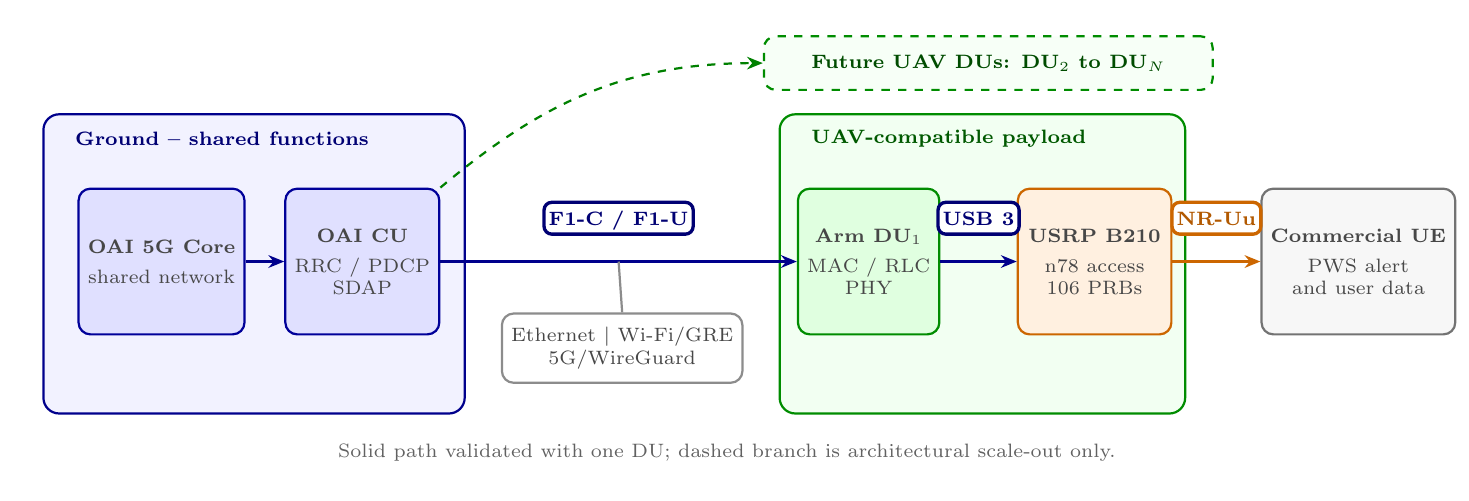
\begin{tikzpicture}[
  x=1cm,
  y=1cm,
  box/.style={thick, rounded corners=1.5mm, align=center,
    font=\scriptsize, text=black!72},
  group title/.style={font=\scriptsize\bfseries, text=blue!45!black,
    anchor=west},
  link badge/.style={draw=blue!45!black, fill=white, rounded corners=1mm,
    inner xsep=0.6mm, inner ysep=0.7mm, outer sep=0pt,
    minimum height=0.38cm, text height=1.45ex, text depth=0.30ex,
    font=\scriptsize\bfseries, text=blue!45!black},
  blue link/.style={draw=blue!55!black, very thick,
    -{Stealth[length=2mm,width=1.6mm]}},
  orange link/.style={draw=orange!80!black, very thick,
    -{Stealth[length=2mm,width=1.6mm]}},
  future link/.style={draw=green!50!black, thick, dashed,
    -{Stealth[length=2mm,width=1.6mm]}}
]
  \path[use as bounding box] (0,0) rectangle (17.95,5.65);

  % Shared ground functions.
  \draw[thick, rounded corners=2mm, draw=blue!55!black, fill=blue!5]
    (0.20,0.75) rectangle (5.55,4.55);
  \node[group title] at (0.48,4.24) {Ground -- shared functions};
  \node[box, draw=blue!60!black, fill=blue!12,
    minimum width=1.90cm, minimum height=1.85cm] (core) at (1.70,2.68)
    {\bfseries OAI 5G Core\\[1mm]shared network};
  \node[box, draw=blue!60!black, fill=blue!12,
    minimum width=1.90cm, minimum height=1.85cm] (cu) at (4.25,2.68)
    {\bfseries OAI CU\\[1mm]RRC / PDCP\\SDAP};
  \draw[blue link] (core.east) -- (cu.west);

  % Validated UAV-compatible payload.
  \draw[thick, rounded corners=2mm, draw=green!55!black, fill=green!5]
    (9.55,0.75) rectangle (14.70,4.55);
  \node[group title, text=green!35!black] at (9.83,4.24)
    {UAV-compatible payload};
  \node[box, draw=green!55!black, fill=green!12,
    minimum width=1.70cm, minimum height=1.85cm] (du) at (10.68,2.68)
    {\bfseries Arm DU$_1$\\[1mm]MAC / RLC\\PHY};
  \node[box, draw=orange!80!black, fill=orange!12,
    minimum width=1.95cm, minimum height=1.85cm] (b210) at (13.55,2.68)
    {\bfseries USRP B210\\[1mm]n78 access\\106 PRBs};

  % F1 bearer and its selectable transports.
  \draw[blue link] (cu.east) --
    node[midway, link badge, yshift=5.5mm] {F1-C / F1-U}
    coordinate[midway] (f1mid) (du.west);
  \node[box, draw=black!45, fill=white, minimum width=2.75cm,
    minimum height=0.88cm] (bearers) at (7.55,1.58)
    {Ethernet $\mid$ Wi-Fi/GRE\\5G/WireGuard};
  \draw[draw=black!45, thick] (bearers.north) -- (f1mid);

  % The dedicated gap keeps the USB label fully visible at print scale.
  \draw[blue link] (du.east) --
    node[midway, link badge, yshift=5.5mm] {USB 3} (b210.west);

  % Commercial handset and radio interface.
  \node[box, draw=black!55, fill=black!3,
    minimum width=1.95cm, minimum height=1.85cm] (ue) at (16.90,2.68)
    {\bfseries Commercial UE\\[1mm]PWS alert\\and user data};
  \draw[orange link] (b210.east) --
    node[midway, link badge, draw=orange!80!black, text=orange!70!black,
      yshift=5.5mm] {NR-Uu} (ue.west);

  % Architectural scale-out, not part of the one-DU validation.
  \node[box, draw=green!55!black, fill=green!3, dashed,
    minimum width=5.70cm, minimum height=0.68cm,
    font=\scriptsize\bfseries, text=green!30!black] (future)
    at (12.20,5.20) {Future UAV DUs: DU$_2$ to DU$_N$};
  \draw[future link] (cu.north east) to[out=40,in=180] (future.west);

  \node[font=\scriptsize, text=black!62] at (8.88,0.25)
    {Solid path validated with one DU; dashed branch is architectural scale-out only.};
\end{tikzpicture}
\caption{Shared-CU testbed architecture.  The solid DU$_1$ path is validated;
the dashed DU$_2\ldots$DU$_N$ branch shows the multi-UAV scale-out direction.
Management traffic stays outside the selected F1 bearer, and packet captures
verify the actual path.}
\label{fig:architecture}
\end{figure*}

The B210 provides up to \SI{56}{\mega\hertz} real-time bandwidth and a
61.44-mega-sample-per-second quadrature path over SuperSpeed USB 3
\cite{ettusb210power}.  The Quectel case uses two independent cells: a donor cell
serves the modem, while the B210 access cell serves the handset.  WireGuard
gives stable F1 endpoint addresses over the modem's dynamic packet session.
This separation prevents the common false positive in which the handset joins
the donor cell while the experiment is attributed to the access DU.

\subsection{Artifact contract and security boundary}

The public artifact~\cite{artifactrepo} tracks the required \texttt{docs/},
safe PWS example, and \texttt{patches/}.  Its manifest gives the full OAI
revision and SHA-256 patch digests; the PWS patch is
\path{patches/sib8/oai-pws-sib8-cu-du.patch}.  A sanitized record maps it to
F1AP handling, DU scheduling, handset observation, rollback, the tested warning
values, and safe log fingerprints.  Pinned historical records corroborate the
configuration lineage and early GRE and 5G/WireGuard gates but are not artifact
inputs.  Runtime inputs, raw logs/captures, credentials, database identifiers,
and keys are excluded.  Prior exposed test values were revoked and replaced,
and publication checks cover Git history and the current tree.

The access B210 and intended handset operate inside the lab Faraday cage on an
isolated test public land mobile network (PLMN), using explicitly test-only
warning text.  A run is invalid if radio containment, the intended UE, the
selected access cell, or exclusive lab ownership cannot be proven.

The operator workflow enforces the sequence below:

\begin{enumerate}
  \item discover the selected host, B210, modem, addresses, routes, USB speed,
  OAI commit, and patch state;
  \item acquire an exclusive operator lock, generate the scenario config, and
  launch the 5GC, CU, transport, and DU in dependency order;
  \item prove core health, F1-C SCTP, F1-U GTP-U, RF synchronization, and the
  absence of F1 leakage onto management interfaces;
  \item separately record handset PWS, registration, PDU session, external
  data network (DN)
  reachability, Internet access, downlink/uplink throughput, and timestamps;
  \item stop all processes, check residue, and reproduce the Ethernet rollback.
\end{enumerate}

This distinction matters: F1 setup and an RF-ready message are machine-side
milestones, not evidence of handset service.  A scenario is accepted only when
the relevant phone-visible gates also pass.

\section{Native AArch64 and Jetson Enablement}

\subsection{Building OAI on Arm}

The working method is a native build on the target, not an x86 binary copied to
the board.  OAI's SIMDe-backed code maps the x86-style vector application
programming interface (API) used throughout the PHY onto AArch64/Neon-compatible implementations
\cite{oaiarmrelease}.  We freeze the same OAI commit on CU and DU, install
dependencies on the Arm host, and build only the required gNB/USRP target:

\begin{verbatim}
git checkout \
  102965a669b9444857c27843ec8ce62780bf9d37
cd cmake_targets
sudo ./build_oai -I
sudo ./build_oai -w USRP --ninja --gNB -C
\end{verbatim}

Four details made this repeatable.  The \texttt{libsctp-dev} and
\texttt{lksctp-tools} packages are installed before the build so compile-time
headers and runtime diagnostics agree.  The USRP Hardware Driver (UHD) and its
B210 images are installed locally; the USB radio cannot be treated as a remote
x86 peripheral.  Build parallelism is bounded and swap is available because
an 8-GB board can otherwise fail during compilation or linking.  Finally, the resulting
\texttt{nr-softmodem}, shared parameter library, UHD backend, and exact source
identity are checked on the target.  No Jetson-specific OAI source fork is
required for AArch64 itself; the lab's PWS and instrumentation changes remain
explicit patches on the pinned tree.

\subsection{Why the stock Jetson kernel failed}

The Jetson Orin Nano ran NVIDIA Linux for Tegra (L4T) R36.4.4 / JetPack 6.2
with kernel
\texttt{5.15.148-tegra}.  The stock configuration contained
\texttt{\# CONFIG\_IP\_SCTP is not set}; \texttt{modprobe sctp} therefore
failed, and creating an SCTP socket returned ``protocol not supported.''  This
blocks both F1-C and any local F1 validation before radio processing starts.

A stand-alone \texttt{sctp.ko} built from generic or mismatched headers was not
a safe fix.  NVIDIA's Board Support Package (BSP) uses out-of-tree Graphics
Processing Unit (GPU), display, audio, and Tegra
drivers.  If the main image, module tree, compiler/configuration, and
\texttt{CONFIG\_LOCALVERSION} disagree, modules fail symbol/version checks; if
the out-of-tree set is omitted, the kernel may boot while graphics and other
board functions fail.

The reproducible fix is published as a separate build artifact
\cite{jetsonkernelrepo}:

\begin{enumerate}
  \item inventory the exact L4T package and stock boot entry;
  \item download the matching R36.4.4 public sources, including in-tree,
  NVIDIA out-of-tree, and display-driver trees;
  \item enable \texttt{CONFIG\_IP\_SCTP=m} and
  \texttt{CONFIG\_INET\_SCTP\_DIAG=m}, and assign an isolated local version;
  \item compile natively with a temporary \SI{4}{\giga\byte} swap file and
  parallelism limited to four jobs, then stage the image and coherent modules;
  \item generate a matching initrd and add, rather than overwrite, an
  \texttt{extlinux.conf} entry so the stock kernel remains selectable.
\end{enumerate}

After reboot, \texttt{checksctp}, a Python SCTP socket, and loopback
\texttt{sctp\_darn} all passed; GPU/display and Ethernet drivers remained
loaded.  This validation is as important as the successful kernel build.

\subsection{Real-time runtime profile}

Kernel support alone did not make the Jetson a stable DU.  At USB 2 speed
(\SI{480}{Mbit/s}), the B210 produced continuous UHD receive overflows.  A
real SuperSpeed path at \texttt{5000M} was necessary but still insufficient.
The validated runtime sets maximum-performance mode, locks clocks, disables
USB autosuspend, sets \texttt{usbfs\_memory\_mb=1000}, runs the DU on CPUs
1--5, and pins the \emph{active} extensible Host Controller Interface (xHCI)
interrupt to CPU 0.  Selecting the active
interrupt by increasing counters, rather than an arbitrary USB-looking line in
\texttt{/proc/interrupts}, removed a repeatability trap.  Warning-level OAI
logging reduces avoidable real-time pressure.

\section{Benchmarks and MCS-Collapse Diagnosis}
\label{sec:benchmarks}

\subsection{Measurement protocol}

The handset was kept on the intended access cell and throughput was accepted
only after PWS, registration, PDU session, and Internet gates.  Interface
captures established whether F1-C and F1-U used Ethernet, GRE, or WireGuard;
for the cellular backhaul case, encrypted outer traffic was also required on
the modem interface.  DU logs supplied MCS, exponentially filtered BLER,
Hybrid Automatic Repeat Request (HARQ) rounds, signal-to-noise ratio (SNR) and
Channel Quality Indicator (CQI) caps, and overflow counts.  Downlink (DL) and
uplink (UL) rates were measured in the handset browser on
\url{https://fast.com}.  Table~\ref{tab:benchmarks}
contains the maximum documented outcome for each row, not means over
identically controlled trials.

\begin{table}[t]
\caption{Maximum documented end-to-end downlink snapshots}
\label{tab:benchmarks}
\centering
\small
\setlength{\tabcolsep}{3pt}
\begin{tabularx}{\columnwidth}{@{}l l l r@{}}
\toprule
DU platform & Architecture & F1 bearer & DL max. (Mb/s) \\
\midrule
x86 reference & Monolithic & local & 190 \\
x86 reference & Split, tuned & Ethernet & 100 \\
x86 reference & Split & Wi-Fi/GRE & 52 \\
x86 reference & Split & 5G/WireGuard & 78 \\
Raspberry Pi 5 & Split & Ethernet & 21 \\
Raspberry Pi 5 & Split & Wi-Fi/GRE & 13 \\
Raspberry Pi 5 & Split & 5G/WireGuard & 48 \\
Jetson Orin Nano & Split & Ethernet & 7.3 \\
Jetson Orin Nano & Split & 5G/WireGuard & 68 \\
\bottomrule
\end{tabularx}
\end{table}

The tuned x86 Ethernet row is the instantaneous peak; the corresponding
sustained result is \SI{89}{\mega\bit\per\second}.  The x86
\SI{78}{\mega\bit\per\second} cellular-backhaul value is the final
researcher-confirmed maximum.  These results establish feasibility across Arm
platforms and bearers.  They do not establish that a tunneled cellular path is
faster than direct Ethernet, which is an intermediate wired reference that may
also be realized over optical fibre.  The final
\SI{68}{\mega\bit\per\second} Jetson 5G/WireGuard record followed a
clean launch with the full MCS range and corrected runtime state.  The artifact
ledger retains the earlier \SIrange{40}{44}{\mega\bit\per\second} configuration
separately, rather than averaging or silently replacing it.

\subsection{Observed mechanism}

The initial Ethernet split plateaued at 12--22 Mb/s with MCS at its configured
floor of 5, although the same access radio could reach high MCS in other
scenarios.  Ethernet identifies the experiment in which the symptom was
isolated; it is not the cause.  Instrumentation of
\texttt{get\_mcs\_from\_bler()} showed OAI applying the filtered estimate

\begin{equation}
\widehat{b}_{k}=0.9\widehat{b}_{k-1}+0.1b_k,
\end{equation}

then incrementing MCS only when \(\widehat{b}_k<b_{\rm lower}\) and
decrementing it when \(\widehat{b}_k>b_{\rm upper}\).  The source defaults
were \((b_{\rm lower},b_{\rm upper})=(0.05,0.15)\).  Under sustained Ethernet
traffic, the measured link showed 22--35\% initial-round HARQ retransmissions and
windowed BLER commonly between 0.18 and 0.40.  The 5\% increment condition was
therefore effectively unreachable, so the controller repeatedly reduced MCS
to the floor.

The direct evidence therefore identifies the BLER-controller mismatch, not
Ethernet capacity, as the dominant observed limiter.  F1-U packetization was
treated as a concurrent transport risk: the after configuration bounded TCP
MSS, but the experiment does not quantify an isolated packet-size effect.  The
same controller behavior can arise on any bearer when its access radio shows a
comparable BLER distribution.

\subsection{BLER retuning and causal scope}

In the after condition, we configured the DU with
\(b_{\rm DL,lower}=0.25\), \(b_{\rm DL,upper}=0.35\),
\(b_{\rm UL,lower}=0.15\), and \(b_{\rm UL,upper}=0.35\).  The radio profile,
attenuation, numerology, Bandwidth Part (BWP), and F1 path were unchanged.
We also clamped new UE TCP sessions to MSS 1360 as a transport guardrail.
Table~\ref{tab:mcs} summarizes the result.

\begin{table}[t]
\caption{Paired wired-split observation for BLER retuning with MSS guardrail}
\label{tab:mcs}
\centering
\small
\begin{tabularx}{\columnwidth}{@{}l X X@{}}
\toprule
Metric & Before & After \\
\midrule
DL target window & 0.05--0.15 & 0.25--0.35 \\
TCP MSS & 1460, no clamp & 1360 \\
Dominant MCS & 5 & 24 and 27 \\
Observed DL BLER & 22--35\% & about 22\% \\
Handset DL & 12--22 Mb/s & 89 Mb/s \\
Instantaneous peak & not accepted & about 100 Mb/s \\
External-DN round-trip time & up to seconds & 11--30 ms \\
\bottomrule
\end{tabularx}
\end{table}

In a five-minute instrumented window after restart, MCS 24 and 27 were the two
most frequent selections; the scheduler was BLER-limited rather than capped by
the MCS table.  The wider target is not a universal optimum: it deliberately
trades more HARQ retransmissions for higher spectral efficiency in this
measured RF condition.  The artifact exposes the thresholds as scenario
parameters and requires new counters before retuning another deployment.

The scheduler trace---filtered BLER above the default target followed by MCS
reduction to the floor---identifies BLER adaptation as the dominant observed
mechanism.  Table~\ref{tab:mcs} is nevertheless not factorial: BLER and MSS
changed together, so the throughput increase belongs to the combined
configuration.  We make no isolated MSS-gain or interaction claim.

\section{Airborne Payload Mass and Mini-Radio Sensitivity}

No aircraft has yet carried the testbed, so the mass model is anchored to the
Jetson, B210, and Quectel configuration that passed attach, PWS, user-plane,
and rollback gates.  Table~\ref{tab:payload} separates measured electronics
from minimum integration allowances; regulated aircraft power yields the
\SI{0.757}{\kilogram} estimate used in the abstract.

\begin{table}[t]
\caption{Validated payload and B200mini board-only projection}
\label{tab:payload}
\centering
\small
\begin{tabularx}{\columnwidth}{@{}X r@{}}
\toprule
Item & Mass (g) \\
\midrule
Jetson Orin Nano board & 151.4 \\
USRP B210 with access antennas & 217.3 \\
Quectel modem kit with antennas & 288.7 \\
\midrule
Measured core electronics & 657.4 \\
Regulator, harness, mounting allowance & 100.0 \\
Validated-radio integration & 757.4 \\
\midrule
B200mini board in place of B210 assembly & 24.0 \\
Projected mini-radio integration$^\ast$ & 564.1 \\
\bottomrule
\end{tabularx}
\vspace{1mm}
\raggedright\footnotesize
$^\ast$Upper-bound mass reduction before adding mini-radio antennas and
enclosure; the B200mini path has not undergone end-to-end validation.
\end{table}

Ettus specifies a \SI{24}{\gram} board-only mass for the B200mini, compared
with the much larger B200/B210 form factor~\cite{ettusb210power}.  Substituting
that board for the measured \SI{217.3}{\gram} B210-and-antenna assembly gives
\(757.4-217.3+24.0=\SI{564.1}{\gram}\).  This is deliberately reported as a
projection: antennas, protection, mounting, and validation can reduce the
\SI{193.3}{\gram} upper-bound saving.  It also explains why the validated
B210 value, rather than the lighter untested radio, remains the headline.

With the engineering rule that payload mass occupy at most 70\% of advertised
capacity, the validated configuration requires at least
\(0.757/0.70=\SI{1.08}{\kilogram}\) of payload rating.  The mini-radio
projection would start at \SI{0.81}{\kilogram} before its missing allowances.
Vehicle selection still requires battery-input, thermal, vibration,
center-of-gravity, electromagnetic-compatibility, and failsafe tests.  A
\SI{50}{\watt} electrical design ceiling is retained for integration, but it
is not presented as a synchronized energy measurement or endurance result.

\section{Conclusion}

Handset-visible single-segment PWS was observed over split F1, with GRE and
early 5G/WireGuard records.  Arm DUs carried data across three F1 bearers.
Jetson delivered \SI{68}{\mega\bit\per\second} over 5G/WireGuard, while the
ledger retains the intermediate \SIrange{40}{44}{\mega\bit\per\second} state.
BLER retuning with an MSS guardrail coincided with MCS 24--27,
\SI{89}{\mega\bit\per\second} sustained, and
\SI{100}{\mega\bit\per\second} peak.  Traces identify the BLER controller as
the dominant observed limiter; no isolated MSS gain is claimed.  The best x86
wireless snapshot was
\SI{78}{\mega\bit\per\second}, versus \SI{30}{\mega\bit\per\second} in the
closest aerial-DU report.  Core electronics weigh
\SI{0.657}{\kilogram}; the \SI{0.757}{\kilogram} integration estimate requires a
\SI{1.08}{\kilogram} payload rating, while an unvalidated B200mini substitution
projects \SI{0.564}{\kilogram}.  One CU can therefore amortize shared functions
across lightweight DUs.  Repeated fixed-condition trials, power measurements,
concurrent DUs, and controlled flight remain future work.

\balance
\bibliographystyle{IEEEtran}
\bibliography{research-paper}

\end{document}
